% +++
% latex = "xelatex"
% +++
\RequirePackage{plautopatch}
\documentclass[12pt,book]{jlreq}
\usepackage[deluxe]{luatexja-preset}
\usepackage{tabularx}
\usepackage[tbtags]{amsmath}
\usepackage[binary-units]{siunitx}
\usepackage{graphicx}
\usepackage{grffile}
\usepackage{fancyhdr}
\setcounter{tocdepth}{3}
\usepackage{newtxtext,newtxmath}
\usepackage{docmute,subfiles}
\usepackage{cleveref}
\usepackage{makeidx}
\usepackage{mathtools}
\usepackage[labelformat=simple,skip=0pt]{subcaption}
\renewcommand\thesubfigure{(\alph{subfigure})}
\usepackage{booktabs}
\aboverulesep=0pt
\belowrulesep=0pt
\usepackage[notrig]{physics}
\usepackage{bm}
\newcolumntype{C}{>{\centering\arraybackslash}X}
\newcolumntype{L}{>{\raggedright\arraybackslash}X}
\newcolumntype{R}{>{\raggedleft\arraybackslash}X}
\renewcommand\index[1]{}
\graphicspath{{figure/}}
\DeclareGraphicsExtensions{.pdf}
% header and footer
\renewcommand{\chaptermark}[1]{\markboth{\thechapter.\ #1}{}}
\pagestyle{fancy}
\fancyhf{}
\renewcommand{\headrulewidth}{0pt}
\fancyhead[LE,RO]{\nouppercase{\thepage}}
\fancyhead[LO]{\sc \nouppercase{\rightmark}}
\fancyhead[RE]{\rm \nouppercase{\leftmark}}
%
\usepackage{tikz}
\usetikzlibrary{matrix}
\usepackage{pgfplots}
\tikzset{% スタイルの作成
  pointtype triangle/.style={mark=triangle*,mark size=4pt},
  every mark/.style={fill=white,solid},
  south west label/.style={
    matrix,matrix of nodes,
    anchor=south west,at={(rel axis cs:0.01,0.01)},
    nodes={anchor=west,inner sep=0},
  },
}
\pgfplotsset{% グラフ全体の見た目の設定
  compat=1.17,
  major tick length=0.2cm,
  minor tick length=0.1cm,
  every axis/.style={semithick},
  tick style={semithick,black},
  legend cell align=left,
  legend image code/.code={%
    \draw[mark repeat=2,mark phase=2,#1]
      plot coordinates {(0cm,0cm) (0.5cm,0cm) (1.0cm,0cm)};
  },
  log number format basis/.code 2 args={
    \pgfmathsetmacro\e{#2}
    \pgfmathparse{\e==0}\ifnum\pgfmathresult>0{1}\else
    \pgfmathparse{\e==1}\ifnum\pgfmathresult>0{10}\else
    {$#1^{\pgfmathprintnumber{\e}}$}\fi\fi},
}
\begin{document}
\frontmatter\relax

\tableofcontents

\chapter{チャプター}

\begin{figure}[b]
  \centering
  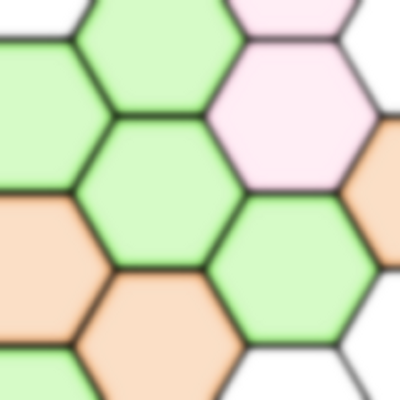
\includegraphics[width=.95\linewidth]{umireon.png}
  \caption{アバター}
\end{figure}

\begin{figure}[b]
  \centering
  \begin{tikzpicture}[thick]
    \begin{semilogyaxis}[% パラメータなどの設定
      width=85mm, height=65mm,
      domain=0:40,
      xmin=0, xmax=40,
      ymin=1e-5, ymax=1,
      minor x tick num=1,
      xlabel={Average CNR $\Gamma$ [dB]},
      ylabel={Bit Error Rate},
      legend entries={Theory,Simulation},
      legend style={draw=none,fill=none},
    ]
      % 理論特性
      \addplot[smooth] gnuplot {(1-1/sqrt(1+2/(10**(x/10))))/2};

      % 復調特性
      \addplot[sharp plot,pointtype triangle,dashed,red] table {data.txt};

      \matrix[south west label] {
        QPSK \\
        Rayleigh fading \\
        Perfect channel estimation \\
      };
    \end{semilogyaxis}
  \end{tikzpicture}
  \caption{グラフ}
\end{figure}

\end{document}
